\subsubsection{Analyse quantitative}
\textbf{Méthodologie}
\smallbreak
D'abord, nous avons évalué la concentration des réserves et de la production du cuivre, du nickel, du lithium, du cobalt, des terres rares et du pétrole, bruts et raffinés. Ainsi, nous avons calculé l'indice Herfindal-Hirschman (HHI) pour chacun d'eux. La formule de cet indice est la suivante :
$$
HHI = \sum_{i=1}^n s_i^2
$$
Avec $n$ le nombre le pays producteurs, et $\forall i \in [1,...,n]$, $s_i$ est la part du pays $i$ dans la production, l'extraction de ressource brute et la production de ressource raffinée. Un HHI situé entre 0 et 1500 dénote une concentration faible, modérée s'il est entre 1500 et 2500, et au-delà, le secteur sera considéré comme hautement concentré.
\smallbreak
Les données utilisées sont tirées des fiches synthèses du BRGM sur la criticité des métaux (\cite{brgm_fiche_2016}),(\cite{brgm_fiche_2016-1}),(\cite{brgm_fiche_2017}),(\cite{brgm_fiche_2018}),(\cite{brgm_fiche_2021}), et du rapport \textit{bp Statistical Review of World Energy} (\cite{bp_statistical_2022}). Pour le pétrole, les données comprennent le pétrole brut, le pétrole de schiste, les sables bitumineux, les condensats (condensats de location ou condensats de gaz qui nécessitent un raffinage supplémentaire) et les LGN (liquides de gaz naturel - éthane, GPL et naphte séparés de la production de gaz naturel).
 En revanche, elles ne comprennent pas les combustibles liquides provenant d'autres sources, comme les biocarburants et les dérivés synthétiques du charbon et du gaz naturel. Sont également exclus les facteurs d'ajustement des combustibles liquides tels que le gain de traitement en raffinerie. Elles excluent également les schistes bitumineux/kérogène extraits sous forme solide.
 Il convient de préciser que les années de référence peuvent différer car les estimations des ressources et de la production des métaux étudiés ne sont pas conduites chaque année. Celles-ci varient donc entre 2016 et 2019 (voir figure \ref{fig:HHI}).
\smallbreak
Ensuite, nous avons comparé le pétrole et les métaux stratégiques susnommés sous l'angle de la stabilité politique. En effet, l'instabilité politique peut être un facteur majeur de conflits, d'accaparation des ressources et autres risques pesant sur la chaîne d'approvisionnement. Pour ce faire, la moyenne de l'indicateur "Stabilité politique et absence de violence/terrorisme" déterminé par la Banque Mondiale a été calculée en la pondérant par la part de chaque pays dans la production et l'extraction. La Banque mondiale définit cet indicateur comme la perception de la probabilité d'instabilité politique et/ou de violence à motivation politique, y compris le terrorisme. Cela prend la forme d'une note entre environ -2,5 et 2,5, la moyenne pour tous les pays du monde étant égale à 0 (voir figure \ref{fig:Polit World Bank}). Ainsi, on peut considérer comme "bon" un score supérieur à 0, et mauvais s'il est inférieur à 0.

\bigbreak
\textbf{Résultats et interprétations}
\smallbreak
\begin{figure}
    \centering
    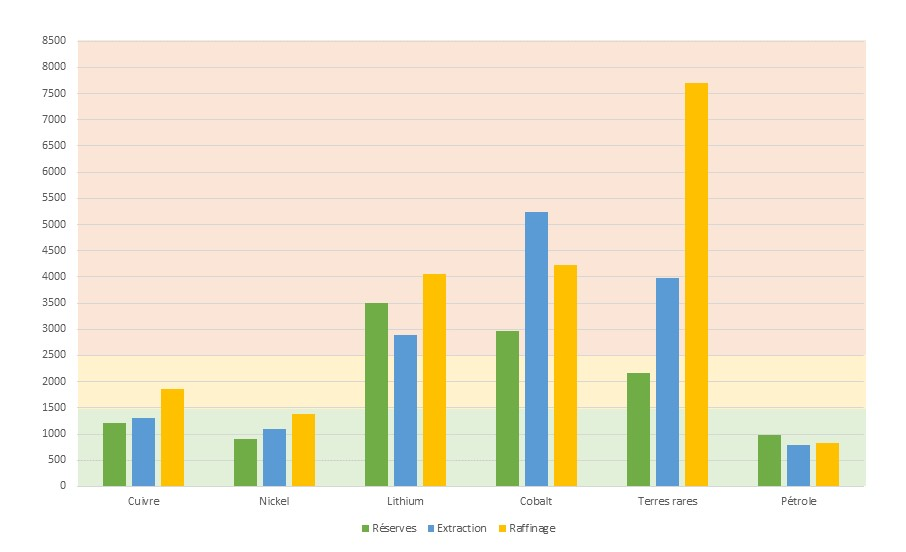
\includegraphics[width=0.8\textwidth]{Images/02 appro/graphe hhi.jpg}
    \caption{Indice Herfindahl-Hirschman des pays extrayant les minerais étudiés et du pétrole. Données tirées de section \ref{section:fiches} ,(\cite{bp_statistical_2022})}
    \label{fig:HHI}
\end{figure}

Sur ce graphe, seuls le pétrole et le nickel ont des réserves, une extraction et une production peu concentrées. Les réserves et l'extraction de cuivre sont peu concentrées, mais sa production l'est modérément. Les autres métaux étudiés ont tous une concentration élevée pour les trois variables, à l'exception des terres rares. En ce qui concerne ces dernières, leur présence géologique dans l'ensemble de la croûte terrestre explique que leurs réserves ne soient que modérément concentrées. Cependant, leur raffinage est particulièrement concentré, tiré par le poids de la Chine malgré une progressive diversification depuis 2010 (voir \hyperref[Chine]{\textit{Les terres rares chinoises : une arme  économique et géopolitique}}). Le HHI bien moins élevé pour le secteur pétrolier que celui des autres ressources étudiées doit cependant être mis en perspective avec le fait que les pays producteurs de pétrole sont géographiquement proches. D'autant plus que la valeur économique des marchés mondiaux de ces métaux est bien moins élevée que celle du marché du pétrole \cite{manberger_geopolitics_2019}.
\smallbreak
Si le cuivre apparaît moins concentré, il faut toutefois souligner que les secteurs qui en dépendent sont nombreux, rendant plus importantes les conséquences industrielles d'une éventuelle rupture d'approvisionnement. Au contraire, les volumes de production bien moindres du cobalt et des terres rares minimisent ces dernières. Le lithium, produits en gros volumes, est plus concentré en comparaison du cuivre, mais des pays de l'OCDE comme le Canada, l'Australie ou encore la France font partie des principaux extracteurs, diminuant de ce fait le risque d'approvisionnement (\cite{brgm_fiche_2017}). 

\begin{figure}
    \centering
    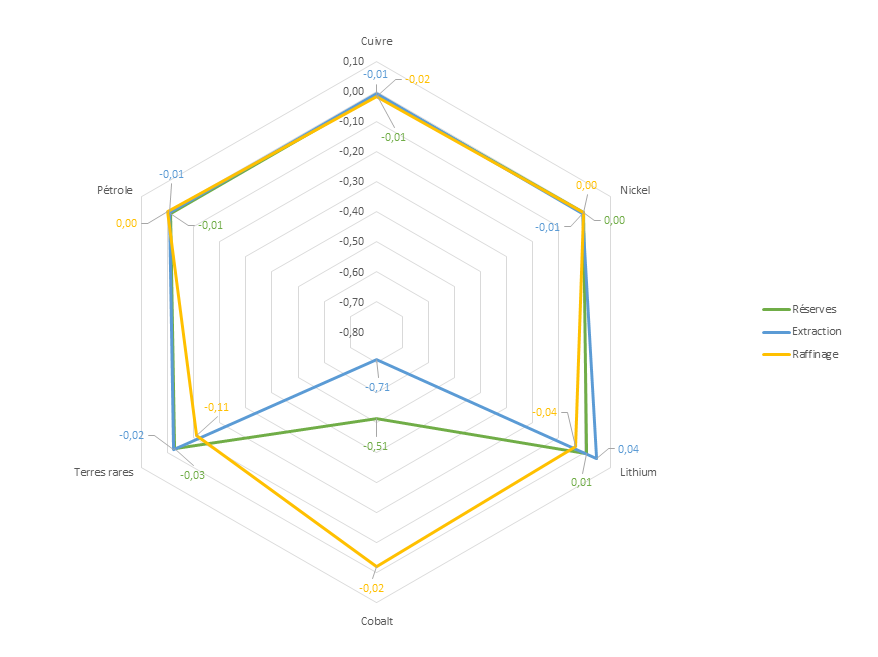
\includegraphics[width=0.8\textwidth]{Images/02 appro/graphe gouvernance.png}
    \caption{Moyenne de l'indice de stabilité politique pondéré par la part de chaque pays dans la production et les réserves de la ressource étudiée. Données tirées de (\cite{world_bank_wgi_2023})}
    \label{fig:Polit World Bank}
\end{figure}
On ne peut pas déduire du calcul de la moyenne de l'indice de stabilité politique que le secteur pétrolier soit plus ou moins vulnérable à l'instabilité et aux violences que ceux du cuivre et du nickel. Toutefois, le score du pétrole tend plus vers la moyenne mondiale que celui des terres rares, du cobalt et du lithium. Une tendance générale est que le secteur du raffinage est moins soumis à l'intabilité, à l'exception des terres rares. Cela peut être expliqué par le fait que les démocraties libérales, mieux notées sur cet indicateur par la Banque mondiale que les régimes autoritaires, ont développé des capacités de raffinage, alors que la transformation des terres rares est toujours dominée par la Chine. La bonne moyenne obtenue par le secteur de la production de lithium brut s'explique par le fait que l'Australie est un acteur majeur de celle-ci, tandis que pour le raffinage la Chine tire le score vers le bas. Quant au cobalt, les scores des réserves et de la production sont si bas en raison la prépondérance de la République Démocratique du Congo. En effet, le pays se relève à peine de la résurgence d'un conflit armé dans les régions de l'Est, qui ont favorisé l'essor du terrorisme. La présence de ressources en cobalt a d'ailleurs pu aggraver ces violences, dans la mesure où ce minéral combine une valeur élevée par poids et volume et la possibilité d'une exploitation minière artisanale (\cite{manberger_geopolitics_2019}).
\smallbreak
\smallbreak
\textbf{Limites et biais}
\smallbreak
Premièrement, la concentration d'un secteur n'est pas nécessairement synonyme de tensions sur la chaîne d'approvisionnement. Un métal peut être très concentré géographiquement mais être produit par des pays qui sont moins susceptibles d'aller à l'encontre des règles du commerce international en perturbant la production ou les exportations de ressources pour leur intérêt national. De plus, les limites entre ce qui est considéré comme peu, modérément et très concentré peuvent être interrogées.
\smallbreak
C'est pourquoi nous avons voulu examiner également l'indice de stabilité pondéré par le poids des pays dans les réserves, la production et l'extraction. Mais cet outil est aussi incomplet. Par définition, étant une moyenne, il est tiré par la note des pays les plus importants dans les réserves et la production. De plus, les indicateurs de la Banque Mondiale sont fondés sur des perceptions d'experts et des populations. La dimension subjective de celle-ci doit donc être prise en compte.
\smallbreak
(\cite{hache_vers_2019}) soulignent d'ailleurs des lacunes dans l'évaluation de la dimension géopolitique de la criticité, dans la prise en compte de l'évolution des restrictions aux importations et dans les recherches empiriques sur le lien entre instabilité politique et disruption des chaînes d'approvisionnement.

\subsubsection{Conséquences en cas de rupture d'approvisionnement}
Au premier abord, les usages captifs du pétrole et des métaux critiques diffèrent de telle sorte que les économies sont plus sensibles à une pénurie ou à une hausse des prix du premier. Une éventuelle crise des approvisionnement pétroliers affecte en premier lieu le secteur des transports, dont sont dépendants non seulement le fret mais également les particuliers. En revanche, une crise affectant un métal contenu dans les batteries de voitures électriques ou des panneaux solaires n'aura pas de conséquence sur les usagers finaux de ces équipements (\cite{iea_role_2021}).
\smallbreak
De même, le secteur de la pétrochimie, qui est le deuxième secteur le plus consommateur de pétrole avec 14\% des consommations totales en 2017, est indispensable aux modes de vie modernes et à la sécurité alimentaire. Il produit notamment les plastiques qui sont le groupe de matériaux en vrac à la croissance la plus rapide du monde. De ce secteur découlent également les engrais azotés de synthèse, qui sous-tendent près de la moitié de la production agricole mondiale (\cite{iea_future_2018}). 
\smallbreak
Une autre différence majeure entre le pétrole et les métaux est que le premier est définitivement brûlé quand il est utilisé, alors que les seconds restent présents dans les infrastructures et les équipements. Cela implique une potentielle récupération et réutilisation grâce au recyclage en fin de vie (voir section \ref{section:maitrise_techno}).
\smallbreak
Ainsi, des disruptions dans les chaînes d'approvisionnement des métaux de la transition énergétique supposeront que celle-ci sera retardée et plus coûteuse, mais elles n'affecteront pas directement les vies quotidiennes des consommateurs (\cite{iea_role_2021}). Néanmoins, elles peuvent constituer de lourdes perturbations sur les industries, et donc entraîner des ralentissements des économies. Par exemple, la mise en place par la Chine de quotas d'exportations de terres rares, suivie d'un embargo non-officiel à l'encontre du Japon (voir encadré \hyperref[Chine]{\textit{Les terres rares chinoises : une arme économique et géopolitique}}), a eu des conséquences sur l'industrie automobile nippone. En septembre 2011, l'entreprise Toyota a annoncé envisager de transférer la fabrication de certains modèles de véhicules hybrides vers la Chine pour éviter lesdits quotas (\cite{niquet_chine_2011}). Cela revêt une importance stratégique dans la course aux brevets pour les technologies bas-carbone et au leadership dans ce secteur.
\smallbreak
Par ailleurs, le pétrole et les minéraux ont en commun que des menaces sur la fiabilité d'approvisionnement peuvent considérablement se répercuter sur les systèmes énergétiques. Dès lors, les préoccupations autour de la sécurité pétrolière sont applicables aux matériaux critiques. Dès lors, la sécurité minérale peut être fondée sur l'expérience retirée des marchés pétroliers. En particulier, comme ce fut le cas pour la sécurité pétrolière, il faut accompagner les mesures sur l'offre d'efforts sur la demande et la résilience : usage de matériaux recyclés, promouvoir une utilisation efficace, évaluer la robustesse des chaîne d'approvisionnement... (voir sections \ref{section:levier} et \ref{section:politiques_publiques}) (\cite{iea_role_2021}).
\bigbreak

\begin{center}
    \boxput*(0,1){
        \colorbox{white}{Les terres rares chinoises : une arme économique et géopolitique}
    }{
    \setlength{\fboxsep}{15pt}
    \fbox{\begin{minipage}{14cm} 

    
« Il y a le pétrole au Moyen-Orient, il y a des terres rares en Chine », aurait dit Deng Xiaoping, initiateur des réformes d’ouverture de l’économie chinoise. Cette citation a un aspect presque prémonitoire, car bien que cela ait évolué depuis (voir section 2.1), en 2011, la République populaire de Chine (RPC) concentrait 50\% des réserves connues et 97,3\% de la production, grâce à son atout-prix. Sa position quasi-monopolistique dans la production de terres rares lui a d’ailleurs servi comme une arme afin d’arriver à ses fins géopolitiques.  \smallbreak
En 2010, un chalutier de pêche chinois et deux bateaux de patrouille des garde-côtes japonais sont entrés en collision en mer de Chine orientale, précisément dans les zones maritimes disputées autour des îles Senkoku/Diaoyu. Cet accrochage a provoqué le contrôle du bâtiment chinois, puis l’emprisonnement de son capitaine au Japon. Suite à cela, la Chine a graduellement réduit ses exportations de terres rares vers le Japon, qui en était alors fortement dépendant : en 2011, 81\% des importations japonaises de ces minerais provenaient de RPC. Celle-ci a nié tout embargo, de façon à éviter une condamnation de l’Organisation Mondiale du Commerce (OMC).  \smallbreak
Cet événement est à mettre en parallèle avec la stratégie chinoise de restriction des exportations de terres rares progressivement mise en place durant les années 2000. En effet, en 2004, la Chine a mis en place de quotas d’exploitation sur les terres rares, de telle sorte qu’en 2006, ses exportations de ces minerais furent divisées par deux. De 2011 à 2012, elle gela officiellement les licences de prospection et d’exploitation. Ces politiques servaient les ambitions de puissances chinoises, car elles permettaient un renforcement du contrôle sur les entreprises étrangères et une promotion des entreprises d’Etat, allant dans le sens du rééquilibrage de la croissance de la RPC vers une industrie à plus forte valeur ajoutée. Cela lui a valu une condamnation par l’OMC en 2014 pour violation des règles du commerce mondiale, à la suite d’une plainte déposée en 2012 par le Japon, les Etats-Unis et l’Union Européenne.  \\
Ces épisodes ont remis au goût du jour la question de la criticité des matériaux dans la stratégie des Etats, et ont renforcé les clivages autour de l’émergence de la puissance chinoise. De ce fait, les pays qui lui étaient dépendants, notamment le Japon, ont depuis développé des contre-stratégies de contournement, par exemple en cherchant d’autres fournisseurs, en constituant des stocks stratégiques ou encore en finançant la recherche. 
\\[0.5cm]
\textit{Sources : \cite{niquet_chine_2011},\cite{lincot_terres_2021},\cite{faujas_matieres_2014}}

    \end{minipage}}
    }
\end{center}
\label{Chine}
~\\
